\documentclass{article}

% Language setting
% Replace `english' with e.g. `spanish' to change the document language
\usepackage[english]{babel}

% Set page size and margins
% Replace `letterpaper' with `a4paper' for UK/EU standard size
\usepackage[letterpaper,top=2cm,bottom=2cm,left=3cm,right=3cm,marginparwidth=1.75cm]{geometry}

% Useful packages
\usepackage{amsmath}
\usepackage{graphicx}
\usepackage[colorlinks=true, allcolors=blue]{hyperref}

\title{Artificial Evolution: Programming a Superior Snake Game AI with Genetic Algorithms}
\author{M. Ibrahim & M. Laursen}

\begin{document}
\maketitle

\begin{abstract}
This paper looks at the enhancement of a neural network controlling a snake in the classic video game "Snake" through genetic algorithms that simulate evolution. Our model successfully outperformed humans in gameplay.
\end{abstract}

\section{Introduction}

In the classic game Snake, the player directs a snake to eat fruits in a confined space, gaining points and increasing the snake's size with each fruit, which complicates gameplay by avoiding collisions with the walls or the snake itself. This paper investigates whether a genetic algorithm, using concepts like mutation and selection, can enhance a computer-controlled snake's performance to match or surpass human players.

\subsection{Research Question/Problem Formulation}

Q1: Using genetic algorithms is it possible to create a snake that can play the game of snake better than the humans in this group?
\newline
Q2: What elements can we tweak in the genetic algorithm to optimize the model?

\section{Methods}

In this study, we used two main techniques to find the best model to solve our problem: Deep Neural Networks (DNN) which is the actual machine learning model, and Genetic Algorithms (GA) to optimize the model.

\subsection{DNN}

Deep Neural Networks (DNNs) are layered machine learning models that mimic the human brain for pattern recognition and complex decision making \cite{cichy2019deep}. Each layer uses activation functions to process inputs and solve non-linear problems, such as playing the game of Snake. DNNs begin with randomized weights and biases, which are refined during training (selection). As we will be using GA, we will describe our way of handling the training of the network, in the following sections.

\subsection{Genetic Algorithms}
Genetic Algorithms (GA) uses principles of evolution, natural selection and genetics. These algorithms operate by simulating the evolutionary process where the most "fit" organism gets to pass on its genes. The GA applies mechanisms such as selection, crossover, and mutation to evolve a population of potential solutions towards the most optimal model.
\newline
\newline
Fitness:
\newline
The fitness scores are used to guide the selection process. By only allowing models with high fitness scores to "reproduce", we can ensure that successful traits are more frequently passed on to the next generations. This selection process is designed to gradually improve the capability of the DNN. \cite{techniquesandparadigms}
\newline
\newline
Selection:
\newline
The process starts with a diverse population, where each individual possesses parameters similar to genetic "DNA". Selection is based on fitness, which determines each individual's probability of contributing to the next generation. Higher fitness individuals are favored, mimicking natural selection where o traits are more likely to be passed on \cite{techniquesandparadigms}.
\newline
\newline
Crossover:
\newline
Crossover combines the selected solutions, allowing for the mixing of genetic material between two individuals. This process creates offspring that inherit traits from the parents, this can lead to new combinations of traits that may perform better than those of any single parent, thereby enhancing the ability of the population to explore and adapt and over time get better to solve complex problems. \cite{techniquesandparadigms}
\newline
\newline
Mutation:
\newline
Mutation introduces random values to the genetic material of an individual, allowing us to have some genetic variation over the generations. By occasionally introducing random values to the DNA, mutation can help the population escape local maxima and continue evolving towards a more optimal solution. \cite{techniquesandparadigms}


\subsection{Data}
The data used in this study are generated dynamically as each model goes through the game environment. Taking a similar approach to \cite{snakeai2020}, the snake's state, which includes its direction, proximity to dangerous elements such as walls or its tail, and it's relative position to food, are converted into a numerical format and used as input to the neural network. 
\newline
\newline
To compare the model with human players, we will collect data from play-throughs by the authors of this paper and compare them to how well the model did.

\section{Analysis}

\subsection{DNN}
In this study, we used a neural network known as "SimpleModel," which consists of four layers: an input layer with 12 nodes, two hidden layers with 14 and 20 nodes, and an output layer with 4 nodes, corresponding to the possible movements (up, down, left, right) of the snake.
\newline
\newline
The initial phase starts with the random assignment of weights and biases across these layers, as described in the methods section. This randomness ensures a varied initial population for the genetic algorithm, facilitating a broad exploration of potential solutions during the early generations. 
\newline
The forward propagation in SimpleModel operates as follows:

\[
\mathbf{y} = \sigma(\mathbf{W} \mathbf{x} + \mathbf{b})
\]
\newline
where \(\mathbf{W}\) represents the weight matrix, \(\mathbf{x}\) is the input vector, \(\mathbf{b}\) is the bias vector, and \(\sigma\) is the tanh activation function used in hidden layers and a softmax in the output layer.

\subsection{Genetic Algorithms}
The  genetic algorithm used in this study is designed to optimize the weights of the DNN through a selection process mentioned earlier, thereby obtaining the most optimal weights for a model tasked with solving the problem of playing a game of snake.
\newline
\newline
\textit{Selection}:
Our selection is a simple strategy where we selected 50\% of the best performing models based on the fitness score. 
To achieve this we created a list to hold the models along side with the fitness score for that specific model. After each generation we sort the list on the fitness score in descending order, and then finally split the list in half to a create  a new list containing the top 50 percent of the models. We can now use this new selection of the best performing model in our population to perform the crossover.
\newline
\newline
\textit{Fitness}:
To create the fitness score its important to understand what problem it is you are solving.
Not only do we want a snake to be able to play the game, we also want it to achieve the highest possible score within a given time limit, which in our case was set to 1500 steps in the game. 
The fitness function for our implementation can be quantified using the following formula:
\begin{equation}
    f = \frac{s}{\log(n + 1)}
\end{equation}
where \( s \) represents the score, and \( n \) represents the number of steps taken. The logarithm is base \( e \), which is the natural logarithm. This formula makes us not penalize longer games less (games with higher steps) due to the logarithmic term in the denominator, while still encourage the model to achieve a high score.
\begin{table}[h!]
    \centering
    \begin{tabular}{ccc} % ccc means 3 columns all centered; adjust as needed
        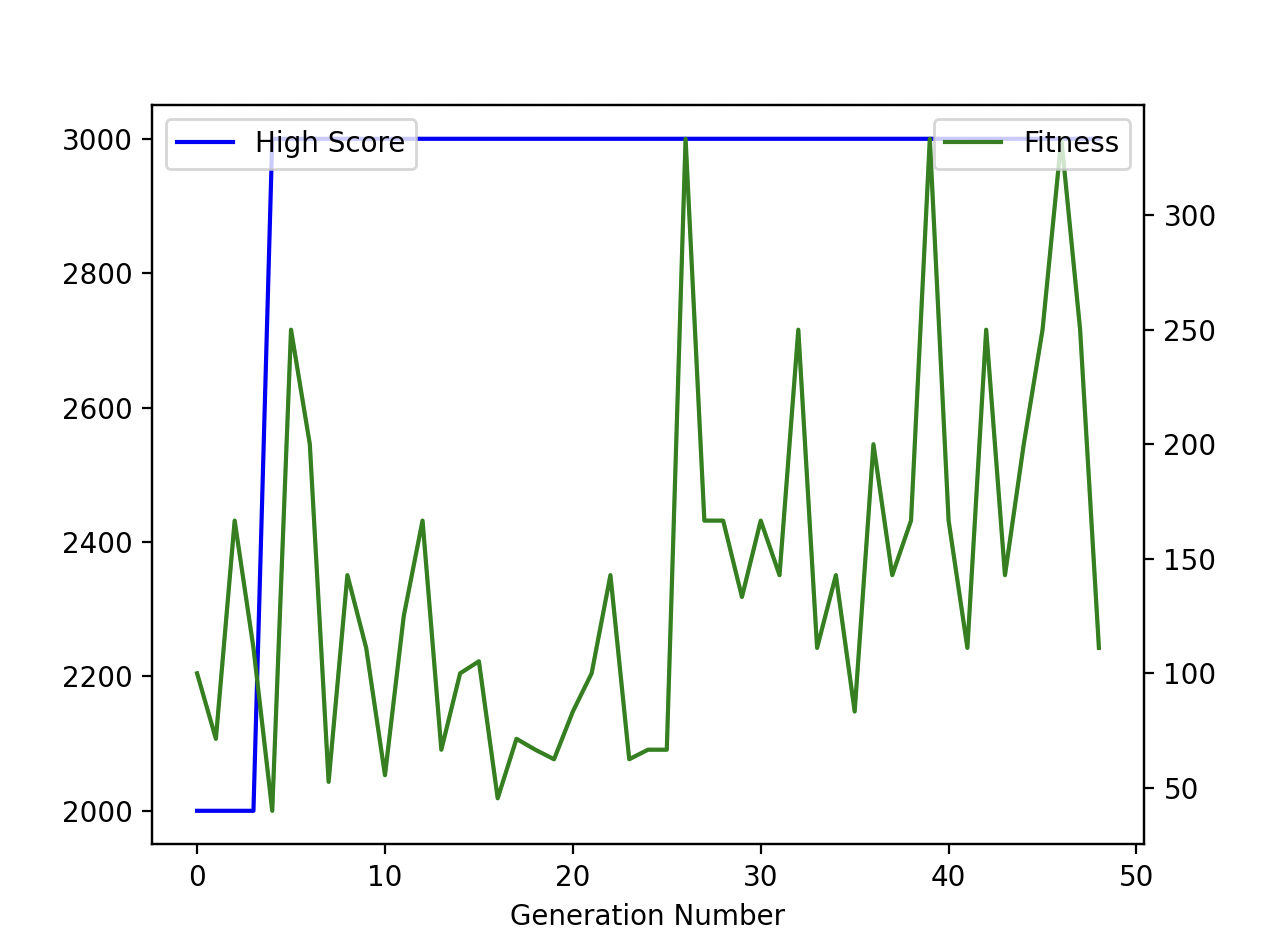
\includegraphics[width=0.3\linewidth]{simple-fitness.png} &
        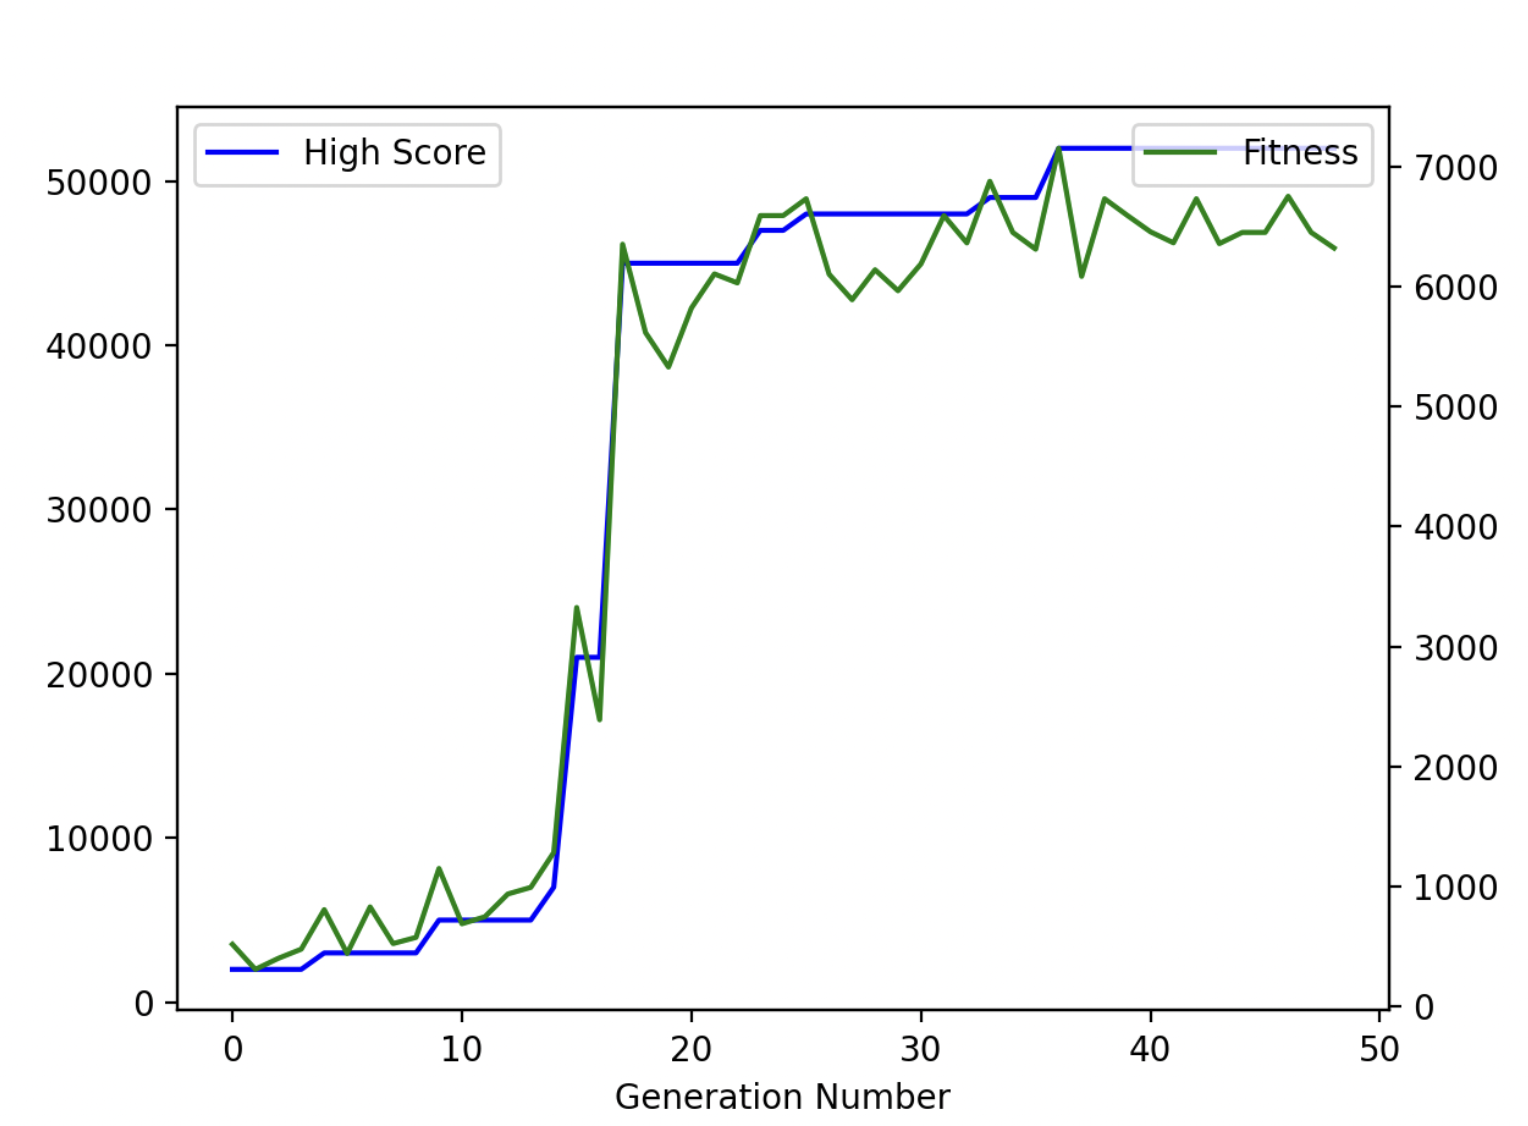
\includegraphics[width=0.3\linewidth]{optimal-settings.png} \\
        \textbf{(a)} Simple fitness score  & 
        \textbf{(b)} Optimized fitness score  \\
    \end{tabular}
    \caption{Comparison of different runs with varying mutation settings.}
    \label{tab:my_label}
\end{table}
\newline
In table 1, we see the difference in how the populations evolve using a simple fitness calculation score (a) where we simply divide the score with the steps, versus how it evolves with the slightly more advanced fitness calculations described earlier (b).
\newline
\newline
\textit{Crossover}:
Once we have the selection, we can now pick two random models from the list, and mix their DNA together mimicking how a new organism is created in nature. 
\begin{figure}[h!]
    \centering
    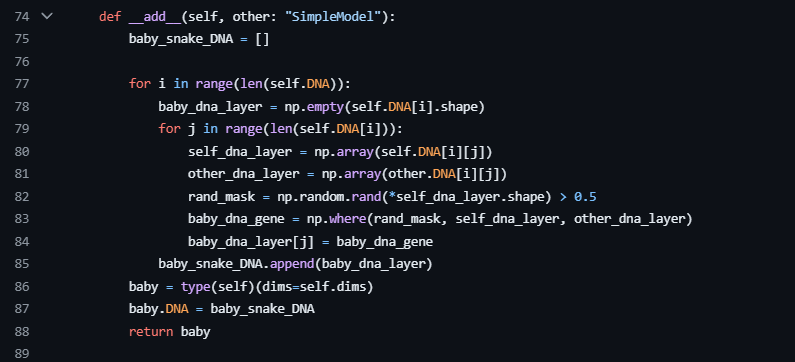
\includegraphics[width=0.3\linewidth]{add-function.png}
    \caption{Crossover function.}
    \label{fig:enter-label}
\end{figure}
\newline
In the figure above, we create the DNA for the "baby snake" by creating a random mask (rand\_mask, figure 1 line 82) consisting of true/false values with the same shape as the current layer that is being iterated through, we then use the "rand\_mask", to create a new DNA string for the baby, this will input values from the parents, the distribution or weights from the selected parents is based on what is true/false in the mask. This gives us a new DNA "genome", that gets appended to its main DNA string.
\newline
\newline
\textit{Mutation}:
For the mutation we could almost reuse the same logic as we used for the crossover. We again create a random mask, with the same shape as the layer we are iterating through but this time we use the models own DNA layer, and a random DNA layer. Using these two layers we create a new layer that is a combination of them (seen below on figure 2).
\begin{figure}[h!]
    \centering
    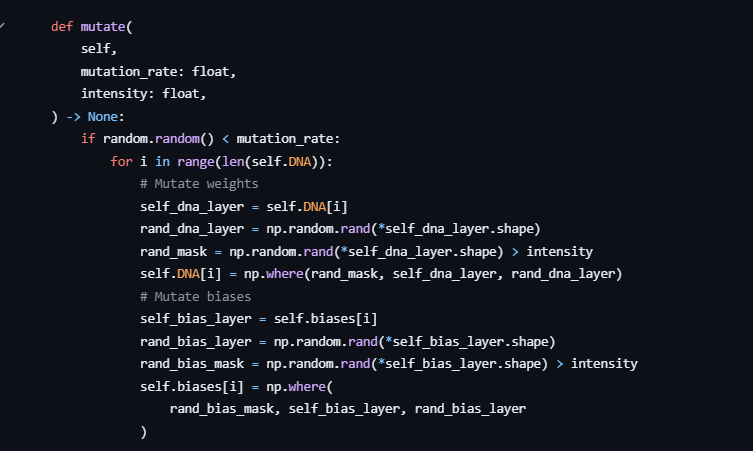
\includegraphics[width=0.3\linewidth]{mutate-function.png}
    \caption{Mutate function}
    \label{fig:enter-label}
\end{figure}
\newline
To be able to have some control over the the impact that the mutation will have on the model, we made the function take two arguments, "mutation\_rate" and "intensity". The mutation rate  controls the chance that a mutation would occur, and the intensity controls how intense the mutation is, in our case it would control how large a chance there is of a weight in the existing DNA gets substituted with a random weight.

\subsection{Data}
The input data for each node is binary (0 or 1), which represents a specific aspect of the snake's environment. A "1" might represent proximity to a wall or the snake's own body, while a "0" might indicate a safe path. This binary input system simplifies the network's processing, since we don't have to normalize any data. 
\newline

As outlined in the methods section, we collected data from games played by the authors of this paper. The data we collected was the score over 5 play-throughs, after a 5-minute warmup period, to reduce outliers. This ensured that each player was accustomed to the game controls, providing more consistent and reliable data.
This data will be used to compare with the GA Snake.




\section{Findings}
\subsection{DNN}

Layers:
To find the optimal amount of layers we had to experiment with sizes of the models, and found that having only one layer, would not make the network "smart" enough to solve the problem and would only reach high scores within the 22.000-25.000 range(table 2, a). We also experimented with adding many layers, but found that 3 layers and up in our DNN, we would need to have more generations for the model to converge (we ran it for 200 generations), but not achieve any noticeable higher score (table 2, b), we achieved a score of around 48.000. The optimal solution for us was having two hidden layers, we could achieve convergence already after 25-30 generation, and achieve a score of about 50.000 (table 2, c). 
\begin{table}[h!]
    \centering
    \begin{tabular}{ccc} % ccc means 3 columns all centered; adjust as needed
        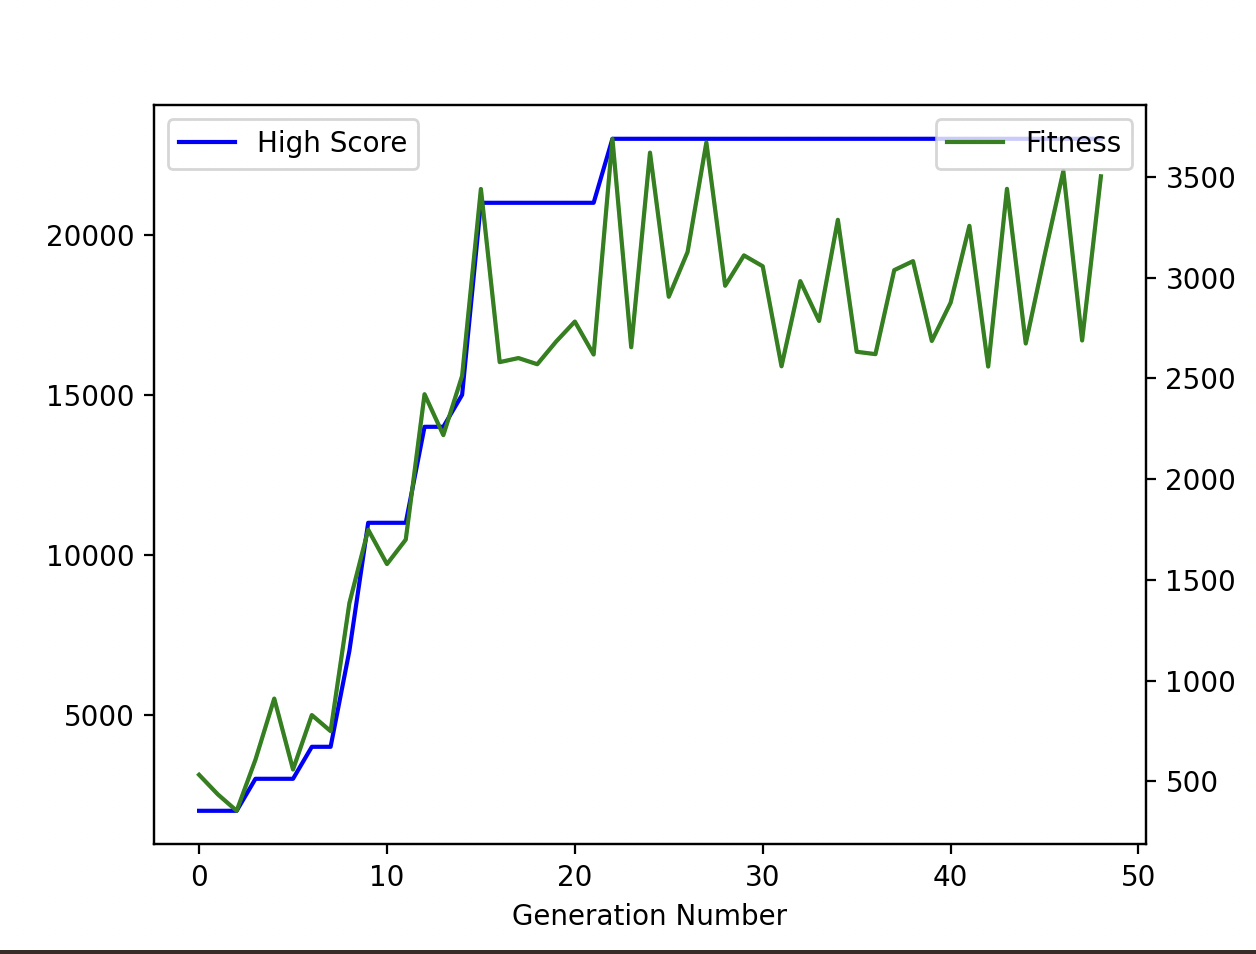
\includegraphics[width=0.3\linewidth]{dnn1layer.png} &
        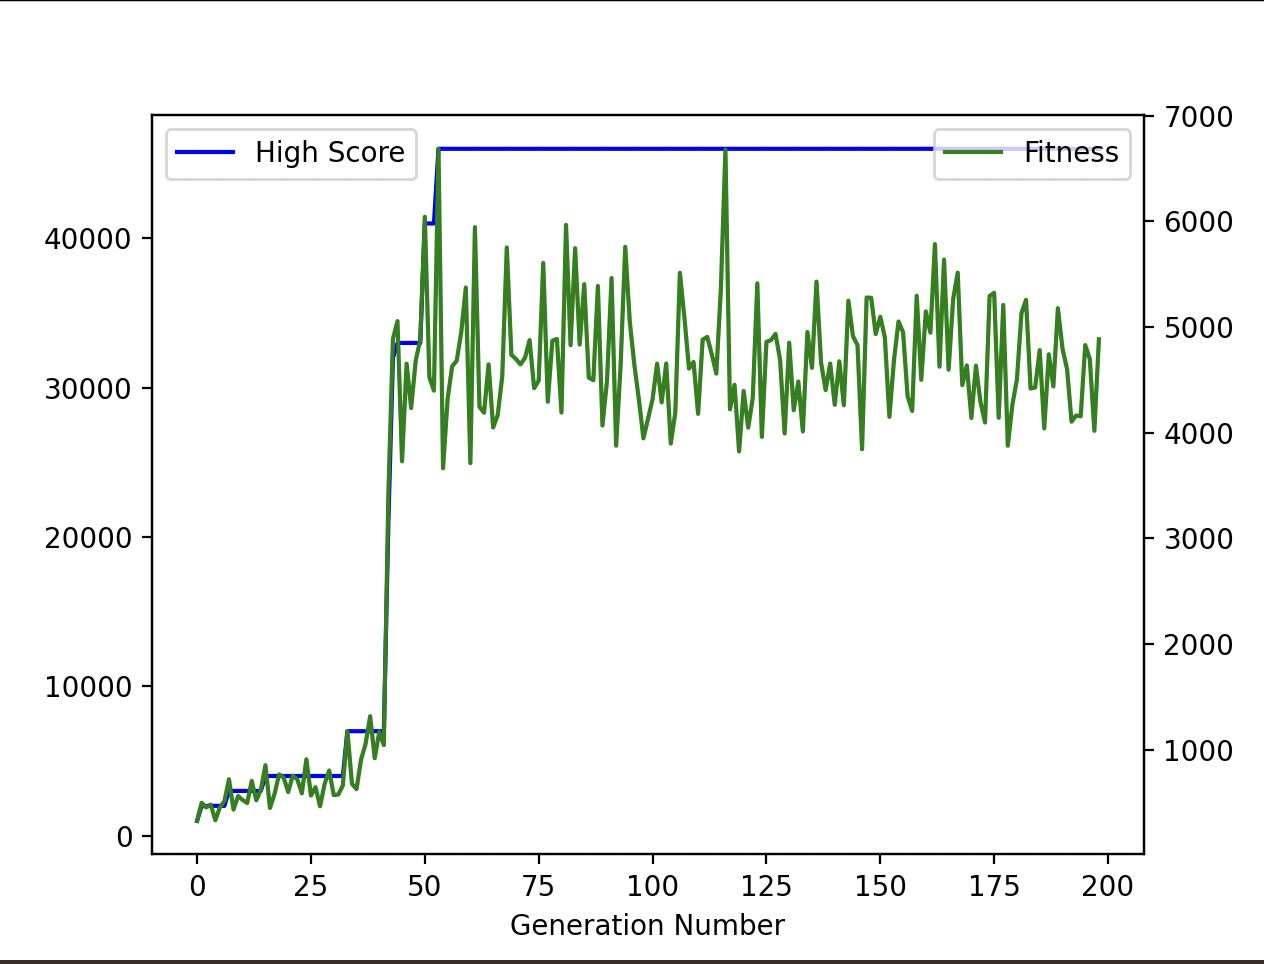
\includegraphics[width=0.3\linewidth]{dnn3layers.png} &
        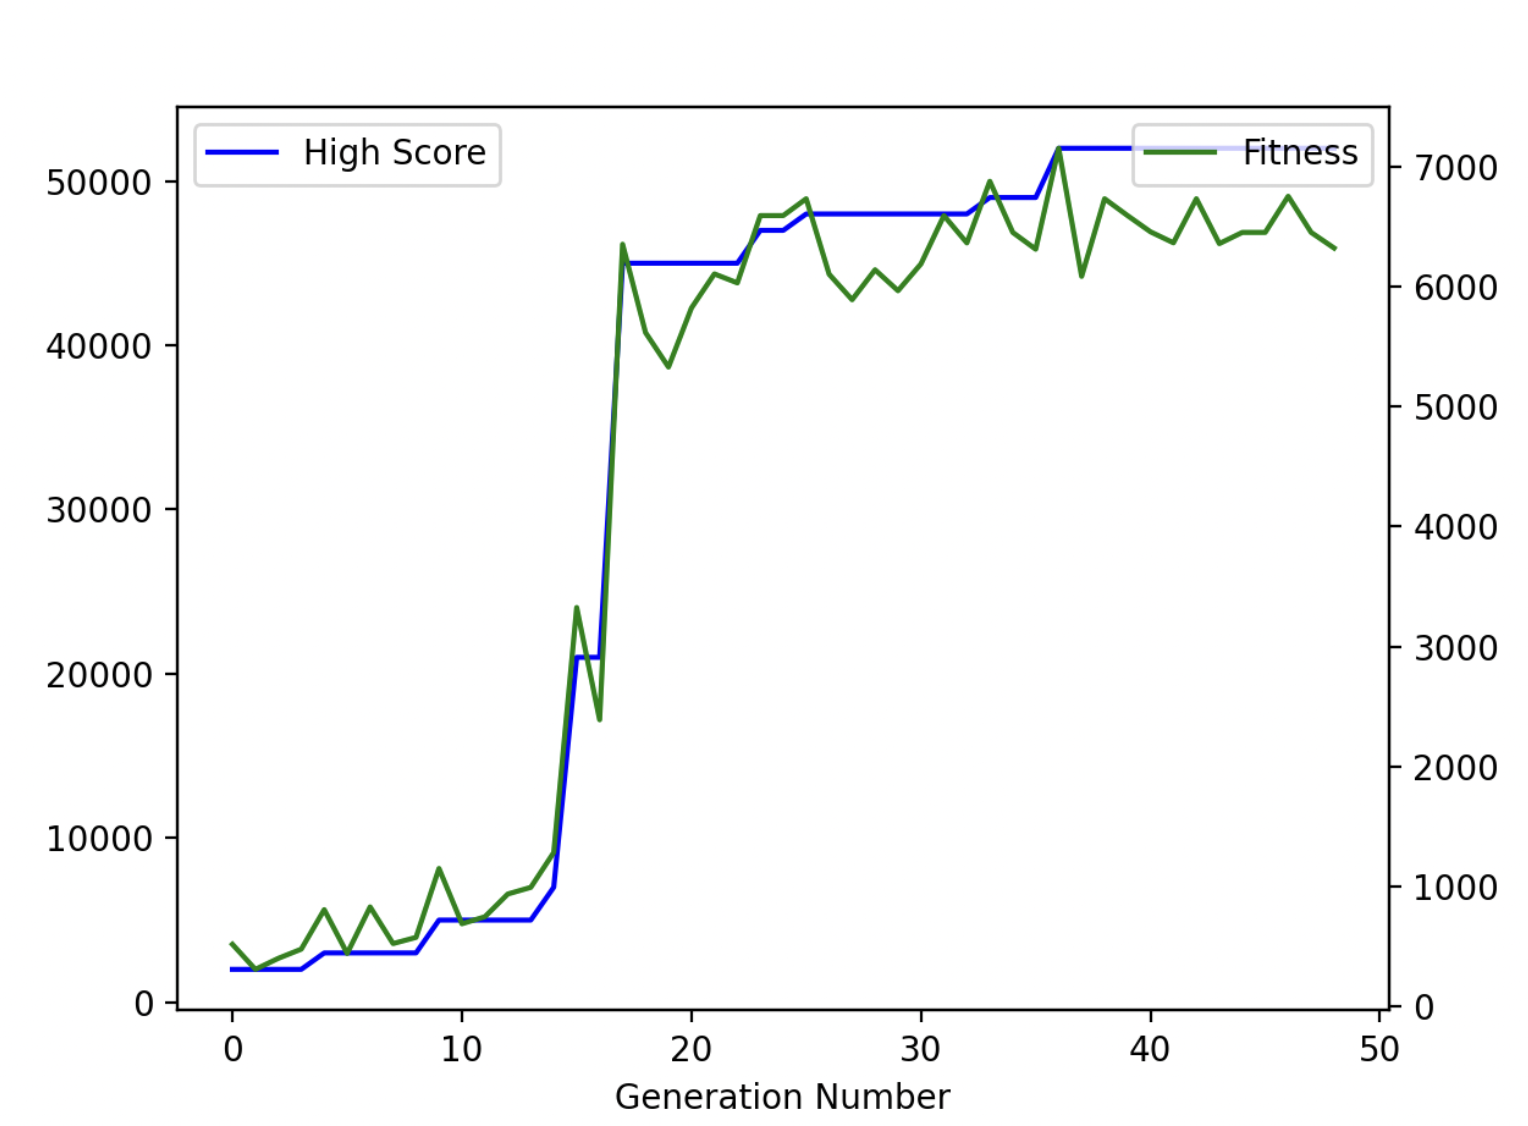
\includegraphics[width=0.3\linewidth]{optimal-settings.png} \\
        \textbf{(a)} DNN one hidden layer & 
        \textbf{(b)} DNN three hidden layers layers  & 
        \textbf{(c)} DNN optimal two hidden layers \\
    \end{tabular}
    \caption{Comparison of different runs with varying mutation settings.}
    \label{tab:my_label}
\end{table}

\subsection{Genetic algorithms\label{gafindings}}

Mutation:
For the mutation, we found that having no mutation would make us hit a maximum early in the run and likely never get over it (Table 3, a), the reason being that no new values would be introduced after the initialization of the first generation, since all offspring would be a mix of these values. 
We also found that having a too high mutation or a too high intensity rate would also cause the model to never find an optimal(Table 3, b) as too many predecessor weights gets replaced with random ones, making the models never evolve.
After experimenting with the values we found that having a mutation rate of 2\%, with an intensity of 10\% was the most optimal, making the model converge fast while still allowing some room for exploration (Table 3, c).
\begin{table}[h!]
    \centering
    \begin{tabular}{ccc} % ccc means 3 columns all centered; adjust as needed
        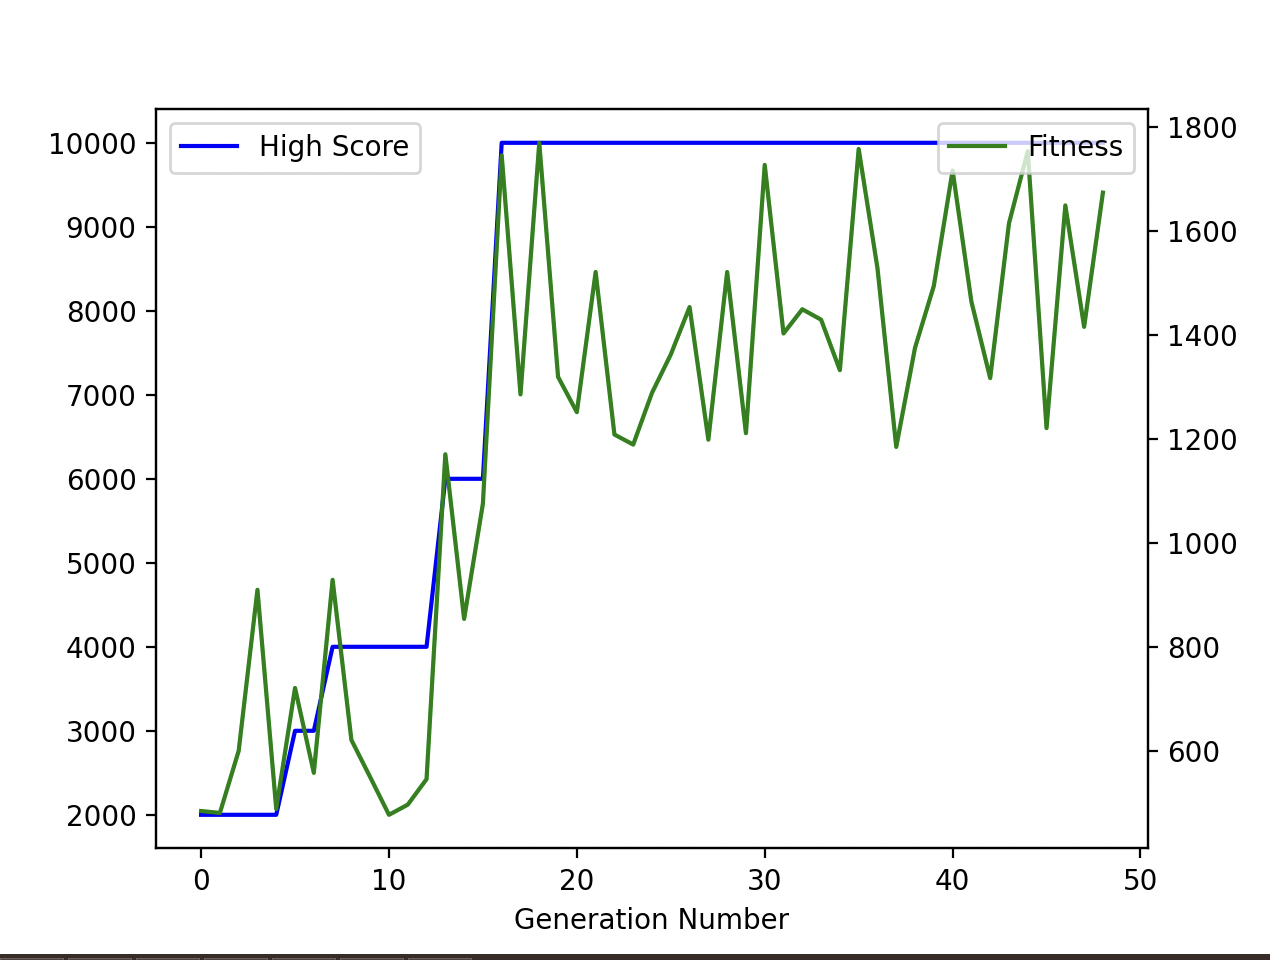
\includegraphics[width=0.3\linewidth]{no-mutation.png} &
        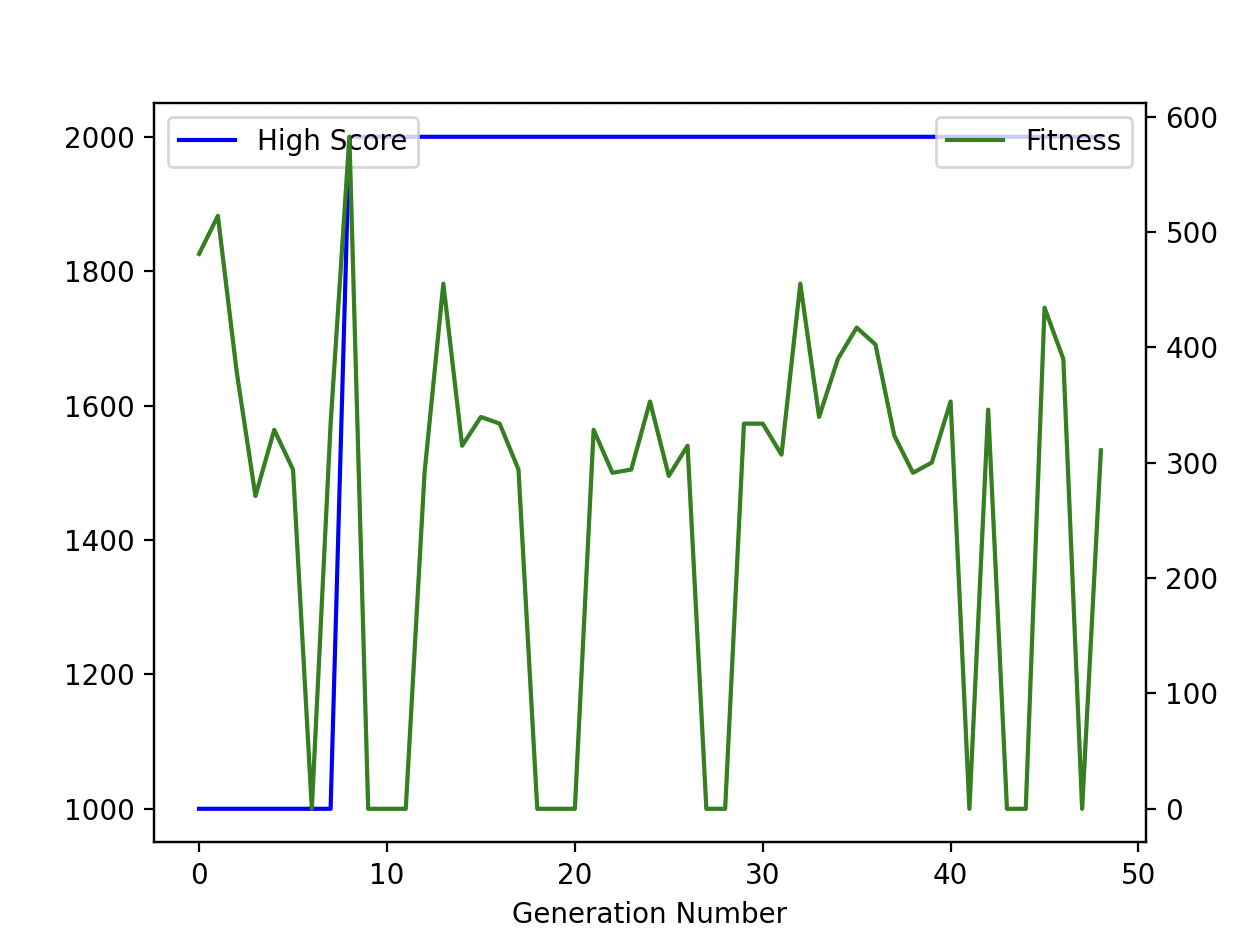
\includegraphics[width=0.3\linewidth]{high_mutation.png} &
        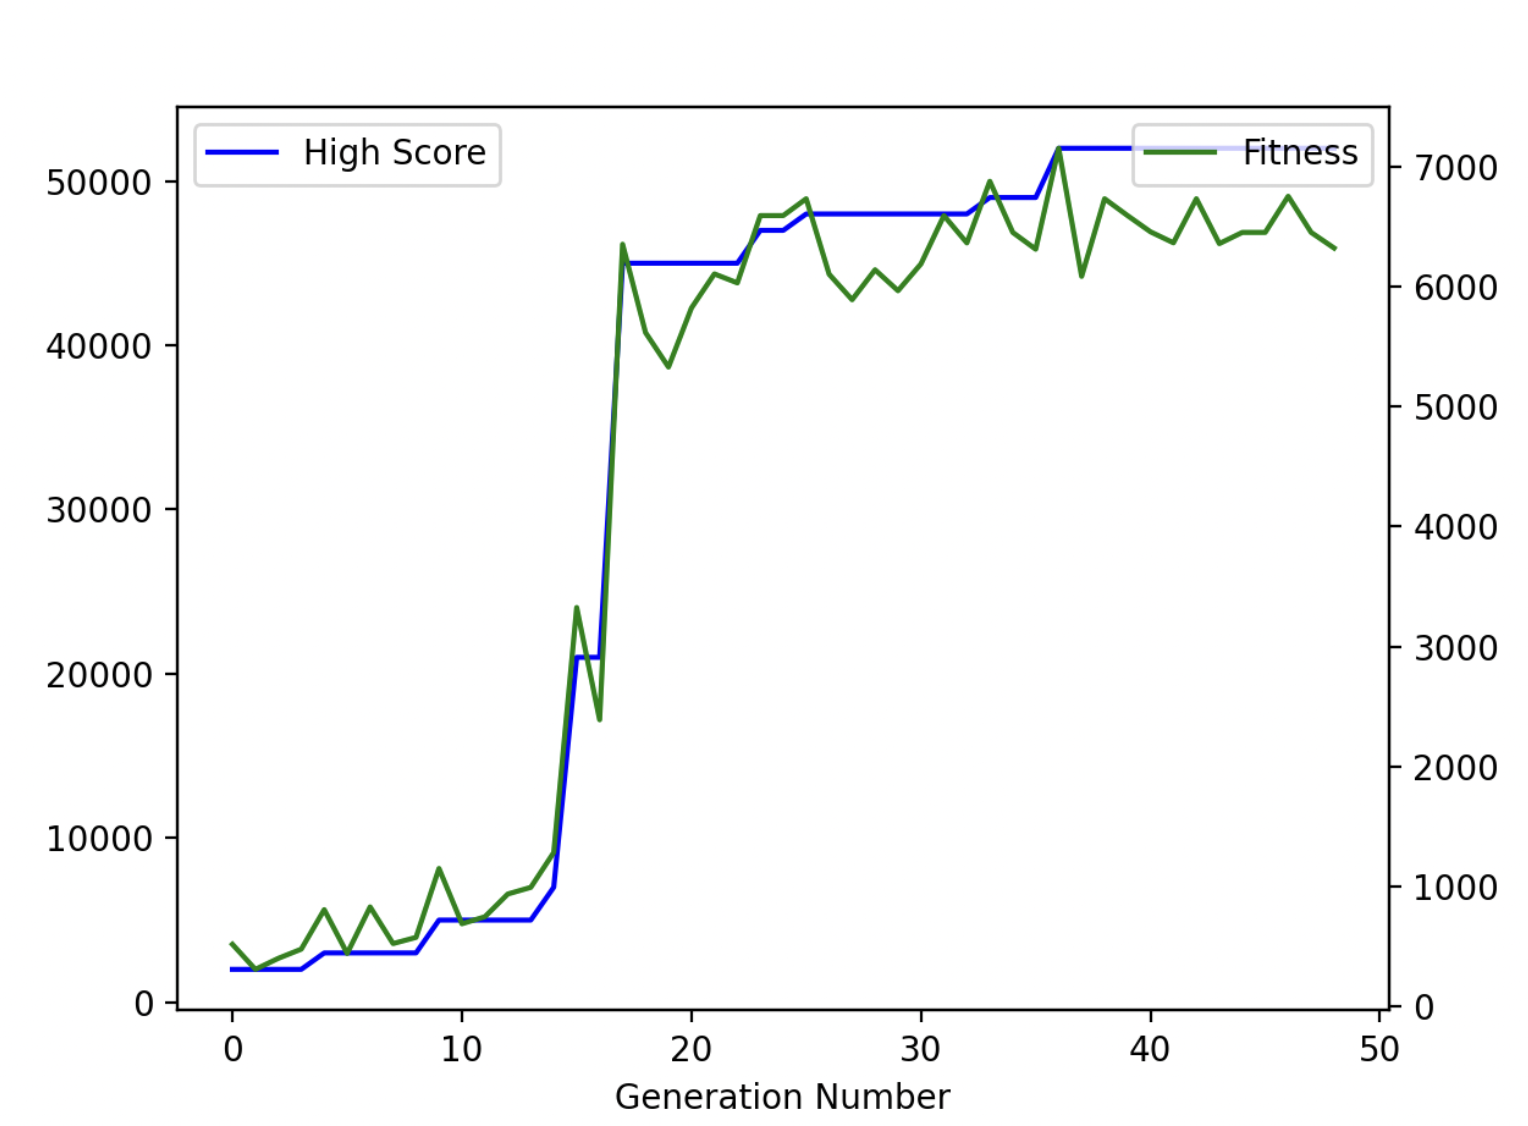
\includegraphics[width=0.3\linewidth]{optimal-settings.png} \\
        \textbf{(a)} No mutation & 
        \textbf{(b)} High mutation  & 
        \textbf{(c)} Optimal run, mutation 2\%, intensity 10\% \\
    \end{tabular}
    \caption{Comparison of different runs with varying mutation settings.}
    \label{tab:my_label}
\end{table}

\subsection{Data\label{datafindings}}


The following table presents the scores of each player over five games, after a 5-minute warmup period.

\begin{table}[h!]
\centering
\begin{tabular}{|c|c|c|c|c|c|}
\hline
\textbf{Player} & \textbf{Game 1} & \textbf{Game 2} & \textbf{Game 3} & \textbf{Game 4} & \textbf{Game 5} \\
\hline
Mohamad & 6000 & 9000 & 9000 & 7000 & 19000 \\
\hline
Martin & 7000 & 16000 & 17000 & 28000 & 7000 \\
\hline
\end{tabular}
\caption{Scores over five games.}
\label{tab:player_scores}
\end{table}

Player 2 achieved the highest score of 28000 points. Comparing this to the highest recorded score of the SimpleModel, which is 58000, it demonstrates that the genetic algorithm was in fact able to out perform human players.
\newline

This also shows that a simple binary input that we used in the models, were effective enough to beat a human.


\section{Conclusion}

To conclude this paper, we will revisit and answer the research questions we asked initially.

Q1: Our findings in \ref{datafindings} indicates that our models outperformed human players, having nearly double the performance. Despite these results, it is possible that with enough practice, a human player could surpass our model in the game of Snake. Additionally, the approach of using only 12 inputs might have limited the models' effectiveness.

Q2: Looking at our findings in \ref{gafindings} shows a fine balance between optimal and subpar model performance. Optimization of the model was achieved by adjusting various parameters such as network sizes, mutation rates, and intensity.


To see the full run over 50 generations: https://www.youtube.com/watch?v=Y1OWveS0Qfw
\bibliographystyle{alpha}
\bibliography{references}


\end{document}




